\sectioncounter{46}

\section{圆锥曲线的综合问题}

\subsection{知识梳理}
圆锥曲线是圆、椭圆、双曲线和抛物线的统称, 它们都可以由平面截圆锥面得到, 后三者可以用焦点、准线和离心率给出统一的定义. 对离心率 $e$, $0<e<1$ 对应椭圆, $e=1$ 对应抛物线, $e>1$ 对应双曲线. 可以认为圆的离心率是 $0$, 这也在一定意义上解释了“离心率”这个词的由来.

对椭圆 $E\colon \dfrac{x^2}{a^2}+\dfrac{y^2}{b^2}=1$ ($a>b>0$), 过焦点 $F(c,0)$ 作 $x$ 轴的垂线, 与 $E$ 交于 $\Big(c,\dfrac{b^2}a\Big)$. 对双曲线 $C\colon \dfrac{x^2}{a^2}-\dfrac{y^2}{b^2}=1$ ($a,b>0$) 也有类似的结论. 此外, $C$ 的焦点到渐近线的距离为 $b$. 了解这些结论对解题有一些帮助.

直线与圆锥曲线相交的问题, 通常要联立两者的方程, 消去 $y$ (或 $x$) 得到关于 $x$ (或 $y$) 的二次方程, 再利用韦达定理 (根与系数的关系) 写出两根满足的式子. 在求面积和弦长等问题中, 常会用到二次方程的两根距离公式. 有时也需要结合圆倠曲线的定义 (即几何特征) 来解题.

\lianxi
\begin{exercise}
    已知双曲线 $C_1\colon \dfrac{x^2}{4}-\dfrac{y^2}{b^2}=1$ 的右焦点 $F_1$ 与抛物线 $y^2 =12x$ 的焦点 $F_2$ 重合, 求双曲线 $C_1$ 的焦点到其渐近线的距离.
\end{exercise}
\beginsolution
    $F_2(3,0)$, 则 $F_1(3,0)$, $b=\sqrt5$, 双曲线 $C$ 的焦点到其渐近线的距离为虚半轴长, 即为 $\sqrt5$.
\endsolution

\begin{exercise}
    已知椭圆 $E\colon \dfrac{x^2}{4}+\dfrac{y^2}3=1$, 双曲线 $C$ 的焦点是椭圆 $E$ 的顶点, 顶点是椭圆 $E$ 的焦点, 求双曲线 $C$ 的离心率.
\end{exercise}
\beginsolution
    双曲线 $C$ 的半焦距为 $2$, 实半轴长为 $1$, 离心率为 $2$.
\endsolution

\begin{exercise}
    设中心在原点的椭圆 $E$ 与双曲线 $C\colon 2x^2 -2y^2 =1$ 有公共的焦点, 且它们的离心率互为倒数, 求该椭圆的方程.
\end{exercise}
\beginsolution
    $C$ 的半焦距为 $1$, 离心率为 $\sqrt2$, 则 $E$ 的半焦距为 $1$, 离心率为 $\dfrac1{\sqrt2}$, 即长半轴长为 $\sqrt2$, 故方程为 $\dfrac{x^2}2+ y^2= 1$.
\endsolution

\begin{exercise}
    若双曲线 $C_1\colon \dfrac{x^2}{a^2}- \dfrac{y^2}{b^2}=1$ 的离心率为 $2$, 抛物线 $C_2\colon x^2=2py$ ($p>0$) 的焦点到双曲线 $C_1$ 的渐近线的距离为 $2$, 求 $p$ 的值.
\end{exercise}
\beginsolution
    设 $C_1$ 的半焦距为 $c$, 则 $\dfrac{c}a= 2$, 即 $c=2a$, $b=\sqrt3a$. 取 $C_1$ 的一条渐近线
    \[l\colon y= \frac{b}a x= \sqrt3 x,\]
    $C_2$ 的焦点为 $\biggl(0,\dfrac{p}2\biggr)$, 作图可知,
    \[\frac{p}2= 2\cdot 2,\quad p=8.\]
\endsolution

\subsection{要点导学\quad 各个击破}
\subsubsection{圆锥曲线的综合问题}
\begin{example}
    已知抛物线 $C\colon y^2 =2px$ ($p>0$) 的焦点为 $F$,  斜率为 $2\sqrt2$ 的直线 $l$ 交 $C$ 于 $A(x_1, y_2)$, $B(x_2, y_2)$ ($x_1<x_2$) 两点, 且 $|AB|=9$.
    
    (1) 求抛物线 $C$ 的方程;\qquad
    (2) 已知 $O$ 为坐标原点, 点 $D$ 为抛物线 $C$ 上一点, 若 $\overrightarrow{OD}= \overrightarrow{OA}+ \lambda\overrightarrow{OB}$, 求 $\lambda$ 的值.
\end{example}
\beginsolution
    $F\biggl(\dfrac{p}2,0\biggr)$, $l\colon y=2\sqrt2\biggl(x-\dfrac{p}2\biggr)$ 与 $C$ 的方程联立,
    \[4x^2- 5px+ p^2=0,\quad x=\frac{p}4,p.\]
    由 $x_1<x_2$ 知, $x_1= \dfrac{p}4$, $x_2=p$, 则
    \[|AB|= \sqrt{1+(2\sqrt2)^2}|x_1-x_2|
    = 3\cdot \frac{3p}{4}= 9,\]
    解得 $p=4$, 所以 $C\colon y^2= 8x$.

    (2) 由 (1) 知, $A(1,-2\sqrt2)$, $B(4,4\sqrt2)$, 并设 $D(2d^2,4d)$, 已知的向量式化为
    \mymarginpar{一般抛物线 $y^2= 2px$ 上的点可以设为 $(2pt^2,2pt)$, 即横坐标和纵坐标均凑成整系数.}
    \[\begin{gathered}
        (2d^2,4d)= (1,-2\sqrt2)+ \lambda(4,4\sqrt2),\\
        2d^2= 1+4\lambda,\quad 4d= -2\sqrt2+ 4\sqrt2\lambda,
    \end{gathered}\]
    消去 $d$ 解得 $\lambda= 0,2$.
\endsolution

\begin{example}
    已知双曲线 $C\colon \dfrac{x^2}{a^2}- \dfrac{y^2}{b^2}=1$ ($a,b>0$) 的左焦点和右焦点分别为 $F_1$,$F_2$, 过点 $F_1$ 的直线与 $C$ 的两条渐近线分别交于 $A$,$B$ 两点, 且 $\overrightarrow{F_1A}= \overrightarrow{AB}$, $\overrightarrow{F_1B}\cdot \overrightarrow{F_2B}= 0$, 求 $C$ 的离心率.
\end{example}
\beginsolution
    由题意, 点 $A$ 为线段 $F_1B$ 的中点, $F1B\perp F_2B$. 作图可知, 点 $A$ 在渐近线 $y=-\dfrac{b}a x$ 上, 点 $B$ 在渐近线 $y=\dfrac{b}a x$ 上. 可设 $A(as,-bs)$. $B(at,bt)$. 又设半焦距为 $c$, 则 $F_1(-c,0)$, $F_2(c,0)$, 所以
    \mymarginpar{本题的难点在于解方程组, 所设点 $A,B$ 坐标的形式可以简化计算, 且求解时应消去辅助量 $s,t$.}
    \[\begin{gathered}
        \frac{-c+at}{2}= as,\quad \frac{0+bt}{2}= -bs,\\
        (at+c)(at-c)+ (bt)^2= 0.
    \end{gathered}\]
    由第二式知, $s=-\dfrac{t}2$, 代入第一式得, $at= \dfrac{c}2$, 再代入第三式,
    \[\frac{3c}2\cdot\biggl(-\frac{c}2\biggr)
    + \biggl(b\cdot \frac{c}{2a}\biggr)^2= 0,\quad
    b^2= 3a^2,\]
    所以 $c^2= 4a^2$, $C$ 的离心率为 $2$.
\endsolution

\begin{example}
    如图 \ref{fig-190629-1540} 所示, 椭圆 $C\colon\dfrac{x^2}{a^2}+\dfrac{y^2}3=1$ ($a>\sqrt3$) 的左顶点、右顶点分别为 $A$,$B$, 离心率 $e=\dfrac12$, 右准线为 $l\colon x=4$, 
    $M$ 为椭圆 $C$ 上不同于 $A$,$B$ 的一点, 直线 $AM$ 与直线 $l\colon x=4$ 交于点 $P$ (在 $x$ 轴上方).
    
    (1) 求椭圆 $C$ 的方程;\qquad
    (2) 若 $\overrightarrow{AM}= \overrightarrow{MP}$, 判断点 $B$ 是否在以线段 $PM$ 为直径的圆上;\qquad
    (3) 连接 $PB$ 并延长, 交椭圆 $C$ 于点 $N$. 若直线 $MN$ 垂直于 $x$ 轴, 求点 $P$ 的坐标.

    \begin{figure}[htb]
        \small
        \centering
        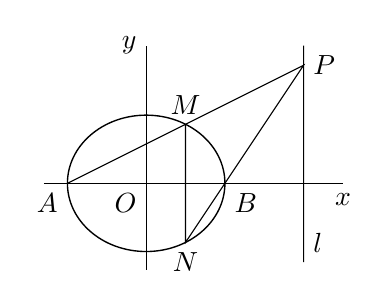
\begin{tikzpicture}[scale=0.5]
          \draw[\myaxisarrow] (-2.6,0) -- (5,0) node[below] {$x$};
          \draw[\myaxisarrow] (0,-2.2) -- (0,3.5) node[left] {$y$};
          
          \draw [line width=0.5pt] (0,0) ellipse (2 and 1.732);
          
          \draw (0,0) coordinate (O) node[anchor=north east] {$O$};
          \draw (-2,0) coordinate (A) node[anchor=north east] {$A$};
          \draw (2,0) coordinate (B) node[anchor=north west] {$B$};
          \draw (4,3) coordinate (P) node[right] {$P$};
          \draw (1,1.5) coordinate (M) node[above] {$M$};
          \draw (1,-1.5) coordinate (N) node[below] {$N$};
          \draw (4,-1.5) coordinate (l) node[right] {$l$};
          
          \draw (A)--(P)--(N)--(M) (4,-2)--(4,3.5);      
        \end{tikzpicture}
        \caption{}\label{fig-190629-1540}
        \end{figure}
\end{example}
\beginsolution
    (1) 设半焦距为 $c$, 则
    \[\frac{c}a= \frac12,\quad a^2= 3+c^2,\]
    解得 $a^2= 4$, 椭圆 $C$ 的方程为 $\dfrac{x^2}4+ \dfrac{y^2}3= 1$.

    (2) 由 (1) 知, $A(-2,0)$, $B(2,0)$. 设 $P(4,p)$, 由 $\overrightarrow{AM}= \overrightarrow{MP}$ 知点 $M$ 为线段 $AP$ 的中点, 则 $M\biggl(1,\dfrac{p}2\biggr)$, 代入 $C$ 的方程得, $p=3$, 即 $P(4,3)$, $M\biggl(1,\dfrac32\biggr)$. 所以
    \mymarginpar{也可以计算点 $B$ 到线段 $PM$ 中点的距离, 并与圆的半径比较.}
    \[\overrightarrow{BM}\cdot \overrightarrow{BP}
    = \biggl(-1,\frac32\biggr)\cdot (2,3)= \frac52,\]
    表明 $\angle PBM$ 为锐角, 因此点 $B$ 不在以线段 $PM$ 为直径的圆上.

    (3) 仍设 $P(4,p)$, 则
    \[PA\colon y= \frac{p}6(x+2),\quad
    PB\colon y= \frac{p}2(x+2).\]
    将 $PA$ 的方程与 $C$ 的方程联立,
    \[(27+p^2)x^2+ 4p^2x+ 4p^2-108= 0,\]
    此方程的两根分别为点 $A,M$ 的横坐标. 设 $M(x_1,y_1)$, 则
    \[(-2)x_1= \frac{4p^2-108}{27+p^2},\quad
    x_1= \frac{54-2p^2}{27+p^2}.\]
    又设 $N(x_2,y_2)$, 同理可得 $x_2= \frac{2p^2-6}{3+p^2}$. 由 $MN\perp x$ 轴知, $x_1=x_2$, 即
    \[\frac{54-2p^2}{27+p^2}= \frac{2p^2-6}{3+p^2},\quad
    p=3,\]
    所以 $P(4,3)$.
\endsolution
    
\lianxi
\begin{exercise}[s]
    已知椭圆 $C\colon \dfrac{x^2}{a^2}+\dfrac{y^2}{b^2}=1$ ($a>b>0$) 上的点到其两个焦点距离之和为 $4$, 且过点 $(0, 1)$.
    
    (1) 求椭圆 $C$ 的方程;\qquad
    (2) 设 $O$ 为坐标原点, 斜率为 $k$ 的直线 $l$ 过椭圆的右焦点 $F$, 且与椭圆交于点 $A(x_1, y_1)$, $B(x_2, y_2)$. 若 $\dfrac{x_1x_2}{a^2}+ \dfrac{y_1y_2}{b^2}=0$, 求 $\triangle AOB$ 的面积.
\end{exercise}
\beginsolution
    (1) $2a=4$, $b=1$, 则 $a=2$, 椭圆 $C$ 的方程为 $\dfrac{x^2}4+ y^2= 1$.

    (2) $F(\sqrt3,0)$, $l\colon y= k(x-\sqrt3)$ 与 $C$ 的方程联立并消去 $y$,
    \[\begin{gathered}
        (1+4k^2)x^2- 8\sqrt3 k^2x+ 12k^2- 4= 0,\\
        x_1+x_2= \frac{8\sqrt3 k^2}{1+4k^2},\quad
        x_1x_2= \frac{12k^2- 4}{1+4k^2},
    \end{gathered}\]
    所以
    \[\begin{aligned}
        y_1y_2&= k(x_1-\sqrt3)(x_2-\sqrt3)\\
        &= k^2[x_1x_2 -\sqrt3(x_1+x_2)+ 3]\\
        &= k^2\biggl(\frac{12k^2- 4}{1+4k^2}
            - \sqrt3\frac{8\sqrt3 k^2}{1+4k^2}+ 3\biggr)\\
        &= -\frac{k^2}{1+4k^2}.
    \end{aligned}\]
    已知等式化为
    \[\frac14\cdot \frac{12k^2- 4}{1+4k^2}- \frac{k^2}{1+4k^2}= 0,\]
    解得 $k^2= \dfrac12$, 则前述 $x$ 的二次方程为 
    \[3x^2- 4\sqrt3x+2= 0,\]
    而
    \[|x_1-x_2|= \frac{\sqrt{\Delta}}{3}= \frac{2\sqrt6}{3}.\]
    因此 $\triangle AOB$ 的面积
    \mymarginpar{在坐标系中求三角形的面积有多种方法, 除了常用的面积公式和面积定理, 还可以用割补法 (如本题).}
    \[\begin{aligned}
        S_{\triangle AOB}&= \frac12|OF|(|y_1|+ |y_2|)
            = \frac{\sqrt3}2{|y_1-y_2|}\\
        &= \frac{\sqrt3}2{|k(x_1-x_2)|}
            = \frac{\sqrt3}2\cdot \frac{\sqrt2}2\cdot \frac{2\sqrt6}3\\
        &= 1.
    \end{aligned}\]
\endsolution

\subsubsection{课堂评价}
\begin{exercise}
    已知双曲线 $C\colon \dfrac{x^2}{a^2}- \dfrac{y^2}{b^2}=1$ ($a,b>0$) 的一条渐近线与直线 $l\colon x+2y-1=0$ 垂直, 求双曲线 $C$ 的离心率.
\end{exercise}
\beginsolution
    取 $C$ 的渐近线 $y=\dfrac{b}a x$. 因为 $l$ 的斜率为 $-\dfrac12$, 则 $\dfrac{b}a\cdot\biggl(-\dfrac12\biggr)= -1$, 故 $b=2a$. 设半焦距为 $c$, 则 $c=\sqrt5a$, 即离心率为 $\sqrt5$.
\endsolution

\begin{exercise}
    已知 $a>b>0$, 椭圆 $C_1\colon \dfrac{x^2}{a^2}+ \dfrac{y^2}{b^2}=1$, 双曲线 $C_2\colon \dfrac{x^2}{a^2}- \dfrac{y^2}{b^2}=1$. 若椭圆 $C_1$ 与双曲线 $C_2$ 的离心率之积为 $\dfrac{\sqrt3}2$, 双曲线 $C_2$ 的渐近线方程.
\end{exercise}
\beginsolution
    设 $C_1$ 的半焦距为 $c_1$, $C_2$ 的半焦距为 $c_2$, 则
    \[\dfrac{c_1}a\cdot \dfrac{c_2}b= \frac{\sqrt3}2,\quad
    4c_1^2c_2^2= 3a^4.\]
    将 $c_1^2= a^2-b^2$, $c_2^2= a^2+b^2$ 代入,
    \[4(a^2-b^2)(a^2+b^2)= 3a^4,\quad a^4= 4b^4,\]
    则 $a=\sqrt2b$. 所以 $C_2$ 的渐近线方程为
    \[y= \pm\frac{b}a x= \pm\frac{\sqrt2}2 x.\]
\endsolution

\begin{exercise}
    已知抛物线 $C_1\colon x^2=2py$ ($p>0$) 与圆 $C_2\colon x^2 +y^2 =1$ 有公切线 $l\colon y=x+b$, 求 $p$ 的值.
\end{exercise}
\beginsolution
    由 $l$ 与 $C_2$ 相切知, 圆心 $(0,0)$ 到 $l$ 的距离为 $1$. 将 $l$ 的方程改写为 $x-y+b=0$, 则
    \mymarginpar{由直线与圆锥曲线相切, 通用的做法是联立两者的方程并消去 $x$ (或 $y$), 所得二次方程有两个相同实根, 即 $\Delta= 0$. 对圆的情形, 常利用圆心到切线的距离等于半径.}
    \[\frac{|b|}{\sqrt{1+1}}= 1,\quad b=\pm\sqrt2.\]
    将 $l\colon y=x+b$ 代入 $C_1$ 的方程, 
    \[x^2- 2px- 2pb=0,\]
    由 $l$ 与 $C_1$ 相切知,
    \[\Delta= (-2p)^2- 4\cdot 1\cdot(-2pb)= 0,\]
    则 $p= -2b= \pm2\sqrt2$.
\endsolution

\subsection{课后练习}
\begin{exercise}
    若抛物线 $C\colon y^2 =2px$ 的焦点 $F_1$ 与椭圆 $E\colon \dfrac{x^2}9+ \dfrac{y^2}5=1$ 的右焦点 $F_2$ 重合, 求抛物线 $C$ 的准线方程.
\end{exercise}
\beginsolution
    $F_2(2,0)$, 则 $F_1(2,0)$, $C$ 的准线方程为 $x=-2$.
\endsolution
    
\begin{exercise}
    已知双曲线 $C_1\colon \dfrac{x^2}{a^2}- \dfrac{y^2}{b^2}=1$ ($a,b>0$) 的左顶点 $A$ 与抛物线 $C_2\colon y^2 =2px$ ($p>0$) 的焦点 $F$ 的距离为 $4$, 且 $C_1$ 的一条渐近线与 $C_2$ 的准线的交于点 $P(-2,-1)$, 求双曲线 $C_1$ 的焦距.
\end{exercise}
\beginsolution
    $A(-a,0)$, $F\biggl(\dfrac{p}2,0\biggr)$, 则
    \[|AF|= a+\frac{p}2= 4.\]
    由已知, $C_1$ 的一条渐近线为 $y= \frac12x$, $C_2$ 的准线为 $x=-2$, 则
    \[\frac{b}a= \frac12,\quad -\frac{p}2= -2,\]
    所以 $p=4$, $a=2$, $b=1$. 故 $C_1$ 的半焦距为 $\sqrt5$, 焦距为 $2\sqrt5$.
\endsolution

\begin{exercise}
    设 $F_1$,$F_2$ 为双曲线 $C\colon \dfrac{x^2}4 \dfrac{y^2}5=1$ 的两个焦点, 点 $P$ 在 $C$ 上且 $|PF_1|:|PF_2|= 2:1$, 求 $\triangle PF_1F_2$ 的面积.
\end{exercise}
\beginsolution
    设 $|PF_1|= 2m$, $|PF_2|= m$. 因为 $C$ 的实半轴长为 $2$, 所以
    \[|PF_1|- |PF_2|= 2m-m= 2\cdot 2,\quad m=4,\]
    则 $|PF_1|= 8$, $|PF_2|= 4$. 而 $C$ 的半焦距为 $3$, 则 $|F_1F_2|= 6$, 由余弦定理, 
    \[\cos\angle F_1PF_2
    = \frac{|PF_1|^2+|PF_2|^2- |F_1F_2|^2}{2|PF_1||PF_2|}
    = \frac{11}{16},\]
    所以 $\sin\angle F_1PF_2= \dfrac{3\sqrt{15}}{16}$, $\triangle PF_1F_2$ 的面积
    \[S_{\triangle PF_1F_2}
    = \frac12|PF_1||PF_2|\sin\angle F_1PF_2
    = 3\sqrt{15}.\]
\endsolution

\begin{exercise}
    设椭圆 $E\colon \dfrac{x^2}{a^2}+ \dfrac{y^2}{b^2}=1$ ($a>b>0$), 双曲线 $C\colon \dfrac{x^2}{m^2}- \dfrac{y^2}{n^2}=1$ ($m,n>0$), 且 $C$ 的两条渐近线与 $E$ 的四个交点及 $E$ 的两个焦点恰为一个正六边形的顶点, 求椭圆 $E$ 和双曲线 $C$ 各自的离心率.
\end{exercise}
\beginsolution
    设 $E$ 的半焦距为 $c$, 则题中正六边形的边长为 $c$. 作图并由正六边形的性质,
    \[2a= c+\sqrt3c,\quad \frac{n}m= \sqrt3,\]
    从而可知 $E$ 的离心率为 $\sqrt3-1$, $C$ 的离心率为 $2$.
\endsolution

\begin{exercise}
    设 $F$ 是椭圆 $E\colon \dfrac{x^2}{a^2}+ \dfrac{y^2}{b^2}=1$ ($a>b>0$) 的左焦点, 过点 $F$ 且倾斜角为 $45^\circ$ 的直线 $l$ 与椭圆 $E$ 相交于 $P$,$Q$ 两点, 且 $|PQ|=\dfrac43 a$.
    
    (1) 求椭圆 $E$ 的离心率;
    
    (2) 设点 $M(0,-1)$ 满足 $|MP|=|MQ|$, 求椭圆 $E$ 的方程.
\end{exercise}
\beginsolution
    (1) 设半焦距为 $c$, 则 $F(-c,0)$, $l\colon y=x+c$, 代入 $E$ 的方程,
    \[\begin{gathered}
        (a^2+b^2)x^2+ 2a^2cx+ a^2(c^2-b^2)= 0,\\
        \Delta= (2a^2c)^2- 4(a^2+b^2)a^2(c^2-b^2)= 8a^2b^4.
    \end{gathered}\]
    设 $P(x_1,y_1)$, $Q(x_2,y_2)$, 则
    \[\begin{aligned}
        |PQ|&= \sqrt{1+1^2}|x_1-x_2|
            = \sqrt2\cdot\frac{\sqrt{\Delta}}{a^2+b^2}\\
        &= \frac{4ab^2}{a^2+b^2}= \frac43a,
    \end{aligned}\]
    所以 $a^2= 2b^2$, 表明 $a^2= 2c^2$. $E$ 的离心率为 $\dfrac{\sqrt2}2$.

    (2) 由 (1) 知, $a^2= 2b^2$, $c=b$, 前述方程化为
    \[3x^2+4cx= 0,\quad x=0,-\frac{4c}3,\]
    此即点 $P$,$Q$ 的横坐标. 不妨设
    \[P(0,c),\quad Q\biggl(-\frac{4c}3,-\frac{c}3\biggr).\]
    又设线段 $PQ$ 的中点为 $N$, 则 $N\biggl(-\frac{2c}3,\frac{c}3\biggr)$, 且由 $|MP|=|MQ|$ 知 $MN\perp PQ$. 因为 $PQ$ 的斜率为 $1$, 所以 $MN$ 的斜率为 $-1$, 结合 $M(0,-1)$ 可解得 $c=3$. 所以椭圆 $E$ 的方程为
    \[\frac{x^2}{18}+ \frac{y^2}9= 1.\]
\endsolution

\begin{exercise}
    过点 $A(0,-1)$ 的直线与抛物线 $C\colon x^2= 2py$ ($p>0$) 交于点 $P$,$Q$, 设 $B(0,1)$, 直线 $BP$ 与 $BQ$ 的斜率分别为 $k_1$ 和 $k_2$. 
    
    (1) 求证: $k_1+k_2= 0$;\qquad
    (2) 若 $k_1k_2= -3$, 求 $\angle PBQ$ 的大小.
\end{exercise}
\beginsolution
    (1) 作图可知, $PQ$ 的斜率存在, 设为 $k$, 则 $PQ\colon y= kx-1$, 代入 $C$ 的方程,
    \[x^2- 2pkx+ 2p= 0.\]
    设 $P(x_1,y_1)$, $Q(x_2,y_2)$, 则
    \[\begin{gathered}
        x_1+x_2= 2pk,\quad x_1x_2= 2p,\\
        k_1= \frac{y_1-1}{x_1}= k- \frac2{x_1},\quad
        k_2= \frac{y_2-1}{x_2}= k- \frac2{x_2},
    \end{gathered}\]
    所以
    \[k_1+k_2= 2k- \frac{2(x_1+x_2)}{x_1x_2}= 2k-2k= 0.\]

    (2) 由 (1) 和 $k_1k_2= -3$ 可设 $k_1= -\sqrt3$, $k_2= \sqrt3$, 则直线 $BP$ 与 $BQ$ 的倾斜角分别为 $120^\circ$ 和 $60^\circ$, 所以 $\angle PBQ= 60^\circ$.
\endsolution